% rubber: onchange qualificacao.acn 'makeglossaries qualificacao'
% rubber: watch qualificacao.acr

% Modelo de qualificação em LaTeX do Mestrado em Ciência da Computação da UECE por Matheus Paixão
% baseado no modelo de dissertação por Rudy Matela.
% Disponível em: https://github.com/mhepaixao/modelo_qualificacao_macc

% Informações para compilação no README.md

\documentclass[pnumabnt,normaltoc,capchap,floatnumber=continuous]{abnt}
\usepackage[bibjustif,abnt-etal-cite=3,abnt-full-initials=yes]{abntcite}
\usepackage{modelo/tex/uece}
\usepackage[toc,page]{modelo/tex/appendix}
\usepackage[portuguese,brazilian,portuges]{babel}
\usepackage[utf8]{inputenc}
\usepackage{abnt-alf}
\usepackage{graphicx}
\usepackage{multicol}
\usepackage{listings}
\usepackage{booktabs}
\usepackage{amsmath}
\usepackage{amsthm}
\usepackage{eucal}
\usepackage{amssymb}
\usepackage{mathrsfs}
\usepackage[order=letter,style=long,acronym,nomain,nonumberlist]{glossaries}
\usepackage{enumitem}
\usepackage{pdfpages}
\usepackage{morefloats}
\usepackage{alltt}
\usepackage{float}
\usepackage{caption}
\bibliographystyle{abnt-alf}

\usepackage[T1]{fontenc}
\errorstopmode

\renewcommand{\ABNTbibliographyname}{Referências}

\DeclareCaptionLabelSeparator{dash}{ -- }
\captionsetup{labelsep=dash}

\hyphenation{com-pu-ta-ção}
\hyphenation{com-bi-na-tó-ria}
\hyphenation{fun-cio-na-li-da-de}

\setcounter{secnumdepth}{3}
\setcounter{tocdepth}{1}

\setlength{\topmargin}{-0.3in}

\local{Fortaleza - Ceará}
\cidade{Fortaleza}
\data{data}

% Informações institucionais
\centro{Centro de Ciências e Tecnologia}
\curso{Mestrado em Ciência da Computação}
\cursosimples{Ciência da Computação}
\instituicao{Universidade Estadual do Ceará}
\instituicaosigla{UECE}
\programa{Programa de Pós-Graduação Acadêmica}


% Descrição para folha de rosto
\comentario{
Proposta de qualificação apresentada ao Curso de Mestrado Acadêmico em Ciência da Computação da Universidade Estadual do Ceará (UECE) como 
requisito parcial para a defesa de dissertação.
}

% Descrição um pouco simplificada (removendo o nome do curso ¬¬)
\comentariosimplificado{
Proposta de qualificação apresentada ao Curso de Mestrado Acadêmico em Ciência da Computação da Universidade Estadual do Ceará (UECE) como 
requisito parcial para a defesa de dissertação.
}

\makeglossaries

% insira os siglas no "glossary.tex"
\newacronym{macc}{MACC}{Mestrado Acadêmico em Ciência da Computação}
\newacronym{uece}{UECE}{Universidade Estadual do Ceará}


% Informações gerais do documento
\autor{Nome Sobrenome}
\autorr{Sobrenome, Nome}
\titulo{Título da Qualificação}
\orientador{Nome do seu Orientador}
%se tiver co-orientador, se não tiver comenta
%\coorientador{Nome do Seu CoOrientador}
% \coorientadordois{Nome do Seu Segundo CoOrientador}

% Membros da comissão avaliadora
\bancaum{Prof. Dr. \ABNTorientadordata\ (Orientador)\\
Universidade Estadual do Ceará -- UECE}

%se tiver co-orientador
%\bancadois{Prof. Dr. \ABNTcoorientadordata (Co-Orientador)\\
%Universidade Estadual do Ceará -- UECE}

%se não tiver co-orientador
\bancadois{Prof. Dr. Membro da Banca\\
Universidade de onde vem o Membro -- Sigla}

\bancatres{Prof. Dr. Membro da Banca\\
Universidade de onde vem o Membro -- Sigla}

% quarto membro da banca, se houver
%\bancaquatro{Prof. Dr. Membro da Banca\\
%Universidade de onde vem o Membro -- Sigla}

% data da defesa
\dataaprovacao{data da defesa}

% Resumo/palavras chaves
\resumotext{
Resumo da qualificação
}
\pcs{Palavra chave 1}{Palavra chave 2}{Palavra chave 3}

% abstract/keywords
\abstracttext{
Abstract
}
\kws{Keyword 1}{Keyword 2}{Keyword 3}

%%%%%%%%%%%%%%%%%%%%%%%%%%%%%%%%%%%%%%%%%%%%%%%%%%%%%%%%%%%%%%%%%%%%%%%%%%%%
% inicio do documento
%%%%%%%%%%%%%%%%%%%%%%%%%%%%%%%%%%%%%%%%%%%%%%%%%%%%%%%%%%%%%%%%%%%%%%%%%%%%

\begin{document}
\capa
\folhaderosto
\termodeaprovacao

% RESUMO - obrigatorio
\begin{resumo}
\noindent\ResumoData
% deixe essa linha em branco

\vspace{1cm}
\noindent
\palavraschave
\end{resumo}
\pagebreak

% ABSTRACT - obrigatorio
\begin{abstract}
\noindent\AbstractData
% deixe essa linha em branco

\vspace{1cm}
\noindent
\keywords
\end{abstract}
\pagebreak

%lista de figuras
\listadefiguras

%lista de tabelas
\listadetabelas

%lista de símbolos, inseridos como glossário
\printglossary[type=\acronymtype,title=Lista de Abreviaturas e Siglas]

% sumario
\renewcommand{\contentsname}{SUMÁRIO}
\tableofcontents

% espaço de um e meio
\onehalfspace


% fim :)



% agora adicione os capítulos
\chapter{Introdução}
\label{chapter:introducao}

Texto da introdução.

Exemplos da utilização de tabelas, figuras e siglas na próxima seção

\section{Objetivos}

Insira os objetivos


\chapter{Revisão Bibliográfica}
\label{revisao_bibliografica}

\section{Figuras}

Para incluir figuras use o seguinte comando:

\begin{figure}[h]
\centering
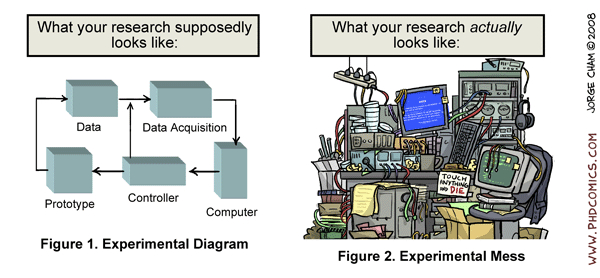
\includegraphics[width=0.6\textwidth]{chapters/fig/research.jpg}
\caption{Legenda da Figura}
\label{label_figura}
\end{figure}

\section{Tabelas}

Pode incluir tabelas usando os ambientes ``table'' + ``tabular'':

\begin{table}[h]
\centering
\caption{Legenda da Tabela usando tabular}
\label{label_tabela_tabular}
\begin{tabular}{||c c c c||} 
\hline
Col1 & Col2 & Col2 & Col3 \\ 
\hline\hline
1 & 6 & 87837 & 787 \\ 
\hline
2 & 7 & 78 & 5415 \\ 
\hline
3 & 545 & 778 & 7507 \\ 
\hline
4 & 545 & 18744 & 7560 \\ 
\hline
5 & 88 & 788 & 6344 \\ 
\hline
\end{tabular}
\end{table}

Também pode usar o ambiente ``table'' e inserir uma tabela como figura:

\begin{table}[h]
\centering
\caption{Legenda da Tabela usando figura}
\label{label_tabela_figura}
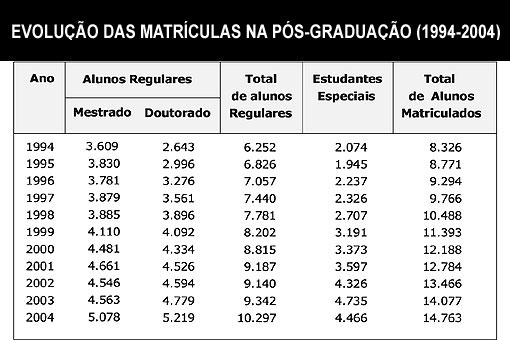
\includegraphics[width=0.5\textwidth]{chapters/fig/tabela.jpg}
\label{label_figura}
\end{table}

\section{Siglas}

Edite o arquivo ``glossary.tex'' com as suas siglas. Veja como exemplo para a sigla do Mestrado Acadêmico em Ciência da Computação da Universidade
Estadual do Ceará.

Este documento é o modelo de qualificação do \acrshort{macc} - \acrshort{uece}

\section{Incluindo referências}

Coloque suas referências no arquivo ``bib.bib'' e cite assim \cite{lamport1986latex}.


% bibliografia
\bibliography{bib}

% caso haja apêndices, use ``\apendice'' antes de inserir
% as secoes
%\apendice
% adicione os apendices, caso existam
%\input{chapters/apendice1}

\end{document}

